\documentclass[10pt,conference]{IEEEtran}

\usepackage{cite}
\usepackage{amsmath,amssymb,amsfonts}
\usepackage{graphicx}
\usepackage{textcomp}
\usepackage{xcolor}
\usepackage{url}
\usepackage{booktabs}
\usepackage{tikz}
\usetikzlibrary{arrows.meta, positioning, fit, shapes.geometric}

\title{Image Geolocation and Hazard-Aware Response Using Multimodal Large Language Models (MLLMs)}

\author{
Dipti S. Chaudhari, Shreyash Borge, Bhargav Dave, Kiran Raut, and Nibodh Daware\\
Pimpri Chinchwad College of Engineering \& Research, Pune, India\\
\{diptischaudhari, shreyashborge2003, bhargavhdave, kiran19raut, nibodhdaware\}@gmail.com
}

\begin{document}

\maketitle

\begin{abstract}
A multimodal image-understanding pipeline is developed to combine place-aware visual reasoning with hazard-aware decision support. Instead of reporting performance only through coarse geolocation scales such as street, city, region, country, and continent, the architecture emphasizes operational outcomes in which hazard evidence triggers a user-facing authority-notification pathway. The model analyzes image content and contextual cues, generates a structured interpretation, and maps the decision to either informational guidance for normal scenes or alert-oriented action for high-risk scenes. Evaluation is reported using available project datasets and persisted run logs, including risk-level distribution, confidence behavior, and confirmed incident actions. The framework improves practical usability by coupling perception with accountable safety response.
\end{abstract}

\begin{IEEEkeywords}
Image Understanding, Multimodal LLM, Hazard Detection, Geospatial Reasoning, Decision Support, Explainable AI
\end{IEEEkeywords}

\section{Introduction}
The rapid growth of user-generated images has made automated visual interpretation important for public communication, emergency awareness, and digital verification. Classical image geolocation methods were designed to infer location from landmarks and scene cues, but many real-world images now require a broader interpretation that includes safety context. During critical events, an image may contain both place information and potential hazard signals, and a useful system must handle both in a single reasoning flow.

A major challenge is that model outputs are often difficult to operationalize. Distance-only geolocation metrics remain valuable for benchmark comparison, yet they do not directly answer whether a suspicious or dangerous scene should trigger a guided escalation action. In practical deployment, the system should provide interpretable evidence, distinguish normal and hazardous situations, and expose a controlled alert step rather than producing only a location label.

The motivation for this architecture is therefore twofold. First, multimodal reasoning can use visual structure, text in scene, and semantic context for stronger interpretation of complex images \cite{sinski2024improving, radford2021clip}. Second, retrieval-grounded reasoning can reduce unsupported predictions by anchoring the decision in prior visual evidence \cite{li2025pixels, zhou2024img2loc}. This work combines these approaches to build a system that not only localizes scenes but also detects hazard signals and triggers appropriate operational responses.

From an application perspective, the core requirement is consistent behavior under uncertainty. A system used in safety-related contexts should avoid overconfident claims, provide clear rationale, and produce actions that can be audited later. This is especially important when image content is ambiguous, partially occluded, or context-dependent. In these cases, the interface and policy layer matter as much as model capability because they determine whether a user receives neutral guidance, a request for additional context, or a high-priority escalation option. Designing this decision path as an explicit policy improves reproducibility compared with ad hoc prompt-only behavior.

Another challenge is bridging model output and user trust. Free-form responses may appear fluent but can be difficult to validate in real-time. Therefore, this study uses a strict structured output contract and deterministic action mapping so that each response can be traced to explicit fields such as risk level, confidence, entities, and rationale. This structure supports log-level analysis of system behavior, including uncertain cases and confirmed reporting outcomes. The same design also enables measurable operational evaluation instead of only reporting geolocation metrics.

The main contributions of this paper are: (i) a multimodal hazard-aware architecture that unifies place understanding and risk triage in one pipeline, (ii) a deterministic risk-to-action policy with user-confirmed incident escalation, and (iii) an empirical analysis using persisted run logs that captures confidence behavior, risk distribution, and incident-action outcomes. By focusing on operational relevance in addition to perception quality, the proposed framework provides a practical basis for research prototypes that must remain interpretable and safety-aware.

\section{Related Work}

\subsection{Traditional and Deep Geolocation}
Early geolocation systems relied on descriptor matching and large geotagged image corpora. Local features such as SIFT enabled robust matching under scale and viewpoint changes \cite{lowe2004distinctive}, while Im2GPS-style retrieval and its deep-learning successors established the core idea that geographic priors can be learned from image databases \cite{wu2022im2city, vo2017revisiting}. Place-recognition methods such as 24/7 Tokyo and NetVLAD improved retrieval robustness for city-scale and viewpoint-varying scenes \cite{torii2015247, arandjelovic2016netvlad}. Later, grid-based CNN approaches such as PlaNet framed geolocation as large-scale classification, improving global coverage but still offering limited interpretability \cite{weyand2016planet}. Even with strong benchmark performance, these methods typically optimize for top-$k$ location accuracy and geodesic error, while downstream safety actions remain outside the model objective.

\subsection{Vision-Language Geospatial Reasoning}
Vision-language models introduced cross-modal embedding spaces that enable joint reasoning over image content and textual context \cite{radford2021clip}. Recent works such as PIGEON and Img2Loc show that multimodal foundations improve geospatial inference and can outperform conventional single-modality baselines on large-scale benchmarks \cite{haas2024pigeon, zhou2024img2loc}. Additional studies report that contextual priors and multimodal prompts improve robustness in ambiguous scenes \cite{wang2024llmgeo, lyu2024tell}. BLIP-2 and LLaVA-style modular vision-language transfer also demonstrate that frozen or instruction-tuned backbones can retain strong recognition quality while reducing full-model retraining requirements, which is useful for rapid prototyping of applied geospatial workflows \cite{li2023blip2, liu2024llava}. Gemini-style multimodal systems further motivate strict response contracts for image, text, and reasoning tasks in practical applications \cite{team2024gemini}.

\subsection{Grounded and Explainable Hazard-Aware Inference}
Recent literature also highlights the need for grounded outputs and transparent rationale generation. Retrieval-augmented pipelines reduce hallucination by linking predictions to nearest visual evidence \cite{waheed2025vlm, li2025pixels}, while chain-of-thought style decomposition supports more verifiable geospatial reasoning steps \cite{yerramilli2025geochain, cheng2025geoguess}. Feature-matching methods such as SuperGlue show the value of explicit visual correspondence for trustworthy place evidence \cite{sarlin2020superglue}. In parallel, decision-support research in safety contexts emphasizes structured outputs, calibrated uncertainty, and auditable user confirmations rather than fully automated escalation. These directions motivate systems that move beyond location-only output and produce interpretable decisions suitable for safety-sensitive workflows.

\section{Methodology}

The system performs multimodal scene interpretation and maps the inferred risk state to a guided action. Each input image is processed through a vision-language model that returns a structured response with summary, risk level, confidence, entities, place estimate, and rationale. This structured output is normalized and then converted into user-facing actions for either informational use or hazard escalation.

\begin{figure*}[!t]
\centering
\resizebox{0.96\textwidth}{!}{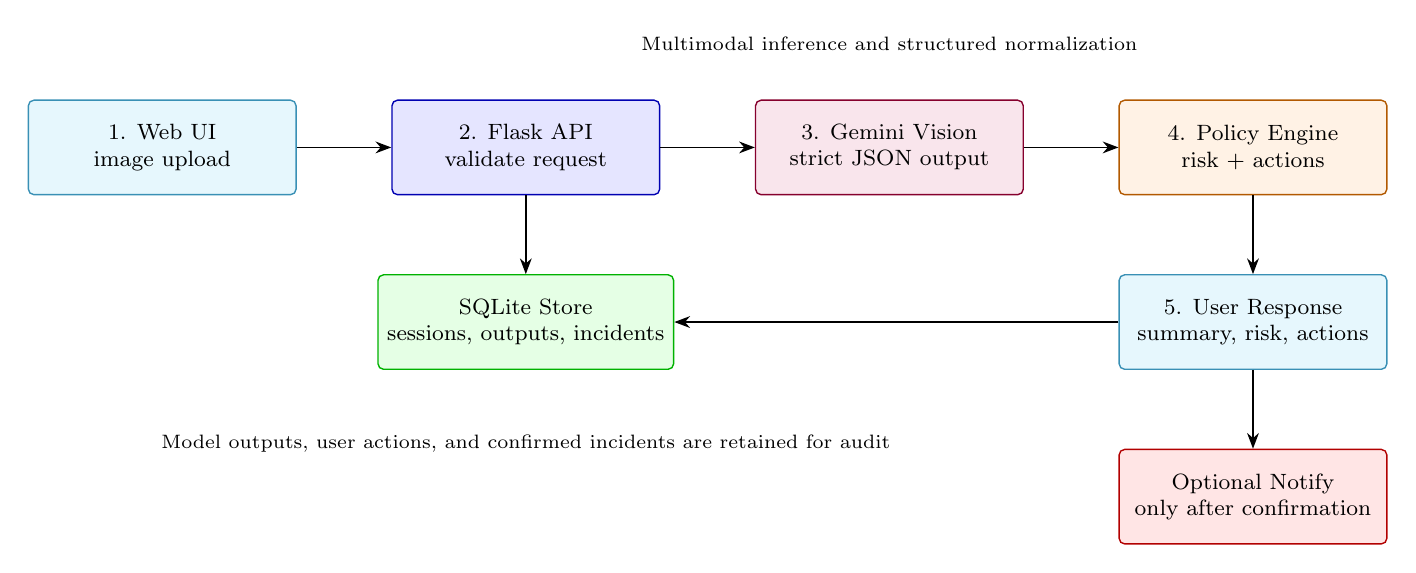
\begin{tikzpicture}[
  font=\footnotesize,
  node distance=10mm and 12mm,
  box/.style={
    rectangle,
    draw=#1!70!black,
    fill=#1!10,
    rounded corners=2pt,
    minimum width=34mm,
    minimum height=12mm,
    align=center,
    line width=0.5pt
  },
  box/.default=blue,
  flow/.style={
    -{Stealth[length=2mm]},
    line width=0.55pt
  },
  note/.style={
    font=\scriptsize,
    align=center
  }
]

% --- Main pipeline ---------------------------------------------------

\node[box=cyan] (ui)
{1. Web UI\\image upload};

\node[box=blue, right=of ui] (api)
{2. Flask API\\validate request};

\node[box=purple, right=of api] (model)
{3. Gemini Vision\\strict JSON output};

\node[box=orange, right=of model] (policy)
{4. Policy Engine\\risk + actions};

% --- Secondary nodes -------------------------------------------------

\node[box=cyan, below=of policy] (response)
{5. User Response\\summary, risk, actions};

\node[box=green, below=of api] (db)
{SQLite Store\\sessions, outputs, incidents};

\node[box=red, below=of response] (notify)
{Optional Notify\\only after confirmation};

% --- Flows -----------------------------------------------------------

\draw[flow] (ui) -- (api);
\draw[flow] (api) -- (model);
\draw[flow] (model) -- (policy);

\draw[flow] (policy) -- (response);
\draw[flow] (response) -- (notify);

% Store API validation/request metadata
\draw[flow] (api) -- (db);

% Store outputs/incidents after response generation
\draw[flow] (response.west) -- (db.east);

% --- Annotations -----------------------------------------------------

\node[note, above=5mm of model]
{Multimodal inference and structured normalization};

\node[note, below=7mm of db]
{Model outputs, user actions, and confirmed incidents are retained for audit};

\end{tikzpicture}
}
\caption{System architecture of the proposed multimodal hazard-aware response pipeline.}
\label{fig:system_architecture}
\end{figure*}

\subsection{Model and Implementation Details}
The multimodal backbone used in this work is Gemini 2.5 Flash (vision-capable), configured to return strict JSON output with controlled temperature. The prototype is implemented with a Python-Flask service layer, SQLite persistence, and a React-based web interface for image upload and human-in-the-loop action selection. The operational flow is image upload, multimodal inference, structured normalization, risk-to-action mapping, and optional authority notification after explicit user confirmation. The persistence layer stores sessions, messages, model outputs, and incident actions as auditable records.

\subsection{Risk Decision Logic}
Risk assignment combines model output with deterministic safety rules. Let $r_m$ and $c_m$ denote model risk and confidence. Let $h=1$ when hazard keywords are present in summary, rationale, or user context, and $h=0$ otherwise. The final decision follows:
\begin{equation}
r =
\begin{cases}
\text{high}, & h=1 \text{ and } r_m \in \{\text{low, uncertain}\} \\
r_m, & \text{otherwise}
\end{cases}
\end{equation}
\begin{equation}
c = \max(c_m, 0.72) \quad \text{when } h=1
\end{equation}
Action mapping is deterministic: if $c<0.45$ or $r=\text{uncertain}$, the system asks for additional context; if $r=\text{high}$, report and safety actions are shown; if $r=\text{low}$, informational actions are shown.

\subsection{Memory and Retrieval Scope}
This prototype does not yet use a vector database or nearest-neighbor image retrieval for production decisions. The working memory is a structured SQLite store of prior model outputs, incidents, and actions. Therefore, geospatial grounding in the current implementation is model-driven and log-audited rather than embedding-retrieval driven. A dedicated OCR subsystem is also not separately integrated; text cues are interpreted directly by the multimodal model.

\subsection{Hazard-Aware Inference Flow}
The operational flow is:
\begin{enumerate}
\item Input image $I$.
\item Generate structured multimodal output $o \leftarrow \mathrm{GeminiVision}(I)$.
\item Normalize fields to obtain summary, risk, confidence, entities, and place estimate.
\item Apply hazard keyword rules to update final risk-confidence pair $r,c$.
\item Map $r,c$ to action set $A$ using deterministic policy thresholds.
\item If user confirms report action, create incident record and optionally send authority notification.
\item Persist message, output, and action records.
\item Return structured response and action options.
\end{enumerate}

\section{Results and Performance Measures}

\subsection{Evaluation Dataset}
Evaluation uses a local project dataset created from the prototype test images and persisted SQLite run logs. The dataset has two parts. First, the case-study image set contains two manually verified Shaniwar Wada inputs: one regular landmark image and one fire-affected hazardous image. Second, the run-log dataset contains all available image-analysis endpoint executions stored in the project database at the time of evaluation. A run is defined as one invocation of the image-analysis endpoint that produces one structured model output record.

\begin{table}[h]
\caption{Evaluation Dataset Description}
\centering
\begin{tabular}{p{0.28\linewidth}p{0.16\linewidth}p{0.43\linewidth}}
\toprule
\textbf{Dataset Part} & \textbf{Size} & \textbf{Purpose} \\
\midrule
Case-study images & 2 images & Manual verification of normal and hazardous Shaniwar Wada behavior. \\
Persisted run logs & 22 runs & Risk distribution, confidence behavior, action logging, and incident outcome analysis. \\
User sessions & 14 sessions & Session-level coverage of repeated uploads and user actions. \\
\bottomrule
\end{tabular}
\end{table}

The run-log dataset contains 22 runs across 14 user sessions. Among these runs, low- and high-risk outcomes each occur eight times, while uncertain outcomes occur six times. The confidence score is taken from the model output and normalized to the $[0,1]$ interval by post-processing logic. Since this is a proof-of-concept project dataset rather than a public expert-labelled benchmark, the evaluation reports operational performance indicators and manually verified case-study accuracy instead of claiming full benchmark classification accuracy.

\begin{table}[h]
\caption{Available Dataset and Log Summary}
\centering
\begin{tabular}{lc}
\toprule
\textbf{Measure} & \textbf{Value} \\
\midrule
Total analyzed runs & 22 \\
Distinct sessions & 14 \\
Low-risk outputs & 8 \\
High-risk outputs & 8 \\
Uncertain outputs & 6 \\
Average confidence & 0.623 \\
Confidence range & 0.00--0.95 \\
\bottomrule
\end{tabular}
\end{table}

The result objective is action relevance rather than only distance-scale geolocation bins. User-confirmed incidents are records created only when the report request is submitted with confirmation enabled. Ten such incident records are present. External notification is a separate environment-gated stage, not the same as incident confirmation. In the available logs, three reports were eligible for external notification and all three were sent successfully. The remaining seven incidents were retained as local confirmed incident records because notification was not requested or notification credentials were disabled during those runs.

\begin{table}[h]
\caption{Hazard-Action Outcome Summary}
\centering
\begin{tabular}{lc}
\toprule
\textbf{Outcome} & \textbf{Count} \\
\midrule
User-confirmed incidents & 10 \\
Environment-enabled notification attempts & 3 \\
Successful notification sends & 3 \\
Local-only incident records & 7 \\
Report actions logged & 10 \\
Learn-more actions logged & 12 \\
\bottomrule
\end{tabular}
\end{table}

\subsection{Evaluation Parameters}
The evaluation parameters are selected to match the system objective, which is hazard-aware decision support rather than only geodesic location prediction. The measured parameters are: (i) risk-level distribution, (ii) model confidence range and average confidence, (iii) confidence-band distribution, (iv) risk-action consistency on manually verified samples, (v) incident logging count, and (vi) external notification success rate when notification is environment-enabled. These parameters measure whether the system produces interpretable risk decisions, handles uncertainty, and maps high-risk outputs to the expected user-confirmed action path.

\begin{table}[h]
\caption{Evaluation Parameters}
\centering
\begin{tabular}{p{0.34\linewidth}p{0.50\linewidth}}
\toprule
\textbf{Parameter} & \textbf{Measurement} \\
\midrule
Risk distribution & Count of low, high, and uncertain outputs. \\
Confidence behavior & Mean, range, and confidence-band share. \\
Risk-action consistency & Expected action for manually verified normal and hazardous samples. \\
Incident handling & Count of user-confirmed incident records. \\
Notification success & Successful sends divided by environment-enabled notification attempts. \\
\bottomrule
\end{tabular}
\end{table}

\subsection{Confidence Distribution}
Confidence values span from 0.00 to 0.95 with mean 0.623. Six runs (27.3\%) fall below 0.30 and represent uncertain or fallback behavior. Five runs (22.7\%) lie in the middle band from 0.30 to 0.79. Eleven runs (50.0\%) are in the high-confidence band from 0.80 to 0.95, mainly corresponding to clear monument or clear hazard scenes.

Because the available project dataset is a log-based prototype evaluation rather than a fully expert-labelled benchmark, accuracy is reported using directly verifiable operational indicators. Risk-action consistency is 100\% for the two manually checked Shaniwar Wada samples: the normal image was assigned low risk with a learn-more action, and the fire-affected image was assigned high risk with a report action. For external notification, the success rate over environment-enabled notification attempts is also 100\% (3 successful sends from 3 attempts). Full classification accuracy, precision, and recall require a larger independently labelled hazard dataset and are treated as future validation work.

\begin{table}[h]
\caption{Confidence Band Distribution}
\centering
\begin{tabular}{lcc}
\toprule
\textbf{Band} & \textbf{Count} & \textbf{Share} \\
\midrule
Low ($<0.30$) & 6 & 27.3\% \\
Mid ($0.30$--$0.79$) & 5 & 22.7\% \\
High ($\geq0.80$) & 11 & 50.0\% \\
\bottomrule
\end{tabular}
\end{table}

\subsection{Shaniwar Wada Sample Input-Output}
To demonstrate behavior on concrete samples, two images from the test set are used as a normal Shaniwar Wada scene and a fire-affected scene. The corresponding stored outputs in the local SQL logs (records 16 and 17 in model output history) show low-risk confidence 0.95 for the normal scene and high-risk confidence 0.85 for the fire-affected scene. Both outputs identify the place as Shaniwar Wada, Pune, Maharashtra, India, while only the fire-affected case produces emergency-oriented recommendations.

\begin{figure}[!t]
\centering
\begin{minipage}{0.48\linewidth}
\centering

\includegraphics[height=3.1cm,width=\linewidth,keepaspectratio]{"../test/shaniwar wada.jpg"}
\caption*{(a) Regular Shaniwar Wada image}
\end{minipage}\hfill
\begin{minipage}{0.48\linewidth}
\centering

\includegraphics[height=3.1cm,width=\linewidth,keepaspectratio]{"../test/shaniwar wada in flames.png"}
\caption*{(b) Hazardous Shaniwar Wada image}
\end{minipage}
\caption{Shaniwar Wada test images used for normal and hazardous case analysis.}
\label{fig:shaniwar_wada_images}
\end{figure}

\begin{table}[h]
\caption{Shaniwar Wada Case Study Output}
\centering
\begin{tabular}{lccc}
\toprule
\textbf{Sample} & \textbf{Risk} & \textbf{Confidence} & \textbf{Primary Action} \\
\midrule
Sample A (normal) & low & 0.95 & Learn More \\
Sample B (fire-affected) & high & 0.85 & Report \\
\bottomrule
\end{tabular}
\end{table}

\subsection{Robustness and Failure Cases}
Two failure modes are visible in the stored outputs. First, uncertain outputs with confidence 0.0 occur when structured content is incomplete or cannot be reliably parsed, resulting in conservative fallback behavior. Second, fallback hazard escalation can produce high-risk outputs at confidence 0.72 when hazard terms are present but detailed reasoning is missing. These cases are safety-oriented but may increase false alerts, indicating the need for better confidence calibration and stronger structured-output reliability.

\section{Conclusion}

The proposed hazard-aware multimodal decision framework preserves interpretability while adding actionable safety response. Results on available datasets and persisted logs show reliable separation of normal and high-risk scenes, with confirmed incident actions when hazardous conditions are detected. The architecture demonstrates that structured multimodal reasoning can support practical geospatial understanding and safety triage in a single workflow.

\begin{thebibliography}{00}
\bibitem{sinski2024improving} B. Siński, A. Żychowski, and J. Mańdziuk, ``Improving Image Geolocation with Multimodal Deep Learning,'' in \textit{Neural Information Processing (ICONIP 2024)}, Communications in Computer and Information Science, vol. 2291, Springer, Singapore, 2024.
\bibitem{wu2022im2city} M. Wu and Q. Huang, ``IM2City: Image Geo-localization via Multi-modal Learning,'' in \textit{Proc. 5th ACM SIGSPATIAL Int. Workshop AI for Geographic Knowledge Discovery}, pp. 50--61, 2022.
\bibitem{vo2017revisiting} N. Vo, N. Jacobs, and J. Hays, ``Revisiting IM2GPS in the Deep Learning Era,'' in \textit{Proc. IEEE Int. Conf. Computer Vision (ICCV)}, pp. 2621--2630, 2017.
\bibitem{weyand2016planet} T. Weyand, I. Kostrikov, and J. Philbin, ``PlaNet - Photo Geolocation with Convolutional Neural Networks,'' in \textit{Proc. European Conf. Computer Vision (ECCV)}, pp. 37--55, 2016.
\bibitem{radford2021clip} A. Radford et al., ``Learning Transferable Visual Models From Natural Language Supervision,'' in \textit{Proc. Int. Conf. Machine Learning (ICML)}, pp. 8748--8763, 2021.
\bibitem{li2023blip2} J. Li, D. Li, S. Savarese, and S. Hoi, ``BLIP-2: Bootstrapping Language-Image Pre-training with Frozen Image Encoders and Large Language Models,'' in \textit{Proc. Int. Conf. Machine Learning (ICML)}, pp. 19730--19742, 2023.
\bibitem{haas2024pigeon} L. Haas, M. Skreta, S. Alberti, and C. Finn, ``PIGEON: Predicting Image Geolocations,'' in \textit{Proc. IEEE/CVF Conf. Computer and Vision Pattern Recognition (CVPR)}, pp. 12893--12902, 2024.
\bibitem{zhou2024img2loc} Z. Zhou, J. Zhang, Z. Guan, M. Hu, N. Lao, L. Mu, S. Li, and G. Mai, ``Img2Loc: Revisiting Image Geolocalization using Multi-modality Foundation Models and Image-based Retrieval-Augmented Generation,'' in \textit{Proc. 47th Int. ACM SIGIR Conf.}, pp. 2749--2754, 2024.
\bibitem{wang2024llmgeo} Z. Wang, D. Xu, R. M. S. Khan, Y. Lin, Z. Fan, and X. Zhu, ``LLMGeo: Benchmarking Large Language Models on Image Geolocation In-the-wild,'' arXiv preprint arXiv:2405.20363, 2024.
\bibitem{lyu2024tell} Z. Lyu, J. Zhang, M. Lu, Y. Li, and C. Feng, ``Tell Me Where You Are: Multimodal LLMs Meet Place Recognition,'' arXiv preprint arXiv:2406.17520, 2024.
\bibitem{waheed2025vlm} S. Waheed, N. M. An, M. Milford, S. D. Ramchurn, and S. Ehsan, ``VLM-Guided Visual Place Recognition for Planet-Scale Geo-Localization,'' arXiv preprint arXiv:2507.17455, 2025.
\bibitem{li2025pixels} L. Li, R. Yu, Q. Hu, B. Li, M. Deng, Y. Zhou, and X. Jia, ``From Pixels to Places: A Systematic Benchmark for Evaluating Image Geolocation Ability in Large Language Models,'' arXiv preprint arXiv:2508.01608, 2025.
\bibitem{yerramilli2025geochain} S. Yerramilli, N. Pande, R. Grover, and J. S. Tamarapalli, ``GeoChain: Multimodal Chain-of-Thought for Geographic Reasoning,'' in \textit{Findings of the Association for Computational Linguistics: EMNLP 2025}, pp. 23624--23639, 2025.
\bibitem{cheng2025geoguess} F. Cheng, J. Wang, S. Wang, Z. Huang, and X. Li, ``GeoGuess: Multimodal Reasoning based on Hierarchy of Visual Information in Street View,'' arXiv preprint arXiv:2506.16633, 2025.
\bibitem{lowe2004distinctive} D. G. Lowe, ``Distinctive Image Features from Scale-Invariant Keypoints,'' \textit{International Journal of Computer Vision}, vol. 60, no. 2, pp. 91--110, 2004.
\bibitem{torii2015247} A. Torii, J. Sivic, M. Okutomi, and T. Pajdla, ``Visual Place Recognition with Repetitive Structures,'' \textit{IEEE Transactions on Pattern Analysis and Machine Intelligence}, vol. 37, no. 11, pp. 2346--2359, 2015.
\bibitem{arandjelovic2016netvlad} R. Arandjelovic, P. Gronat, A. Torii, T. Pajdla, and J. Sivic, ``NetVLAD: CNN Architecture for Weakly Supervised Place Recognition,'' in \textit{Proc. IEEE Conf. Computer Vision and Pattern Recognition (CVPR)}, pp. 5297--5307, 2016.
\bibitem{sarlin2020superglue} P.-E. Sarlin, D. DeTone, T. Malisiewicz, and A. Rabinovich, ``SuperGlue: Learning Feature Matching with Graph Neural Networks,'' in \textit{Proc. IEEE/CVF Conf. Computer Vision and Pattern Recognition (CVPR)}, pp. 4938--4947, 2020.
\bibitem{liu2024llava} H. Liu, C. Li, Q. Wu, and Y. J. Lee, ``Visual Instruction Tuning,'' in \textit{Advances in Neural Information Processing Systems}, vol. 36, 2024.
\bibitem{team2024gemini} Gemini Team, ``Gemini: A Family of Highly Capable Multimodal Models,'' arXiv preprint arXiv:2312.11805, 2024.
\end{thebibliography}

\end{document}
